\paragraph{}This chapter goes over 2 examples of tuning 2 distinct \ac{SLAM} algorithms(faster-lio and fast-livo2), using all three tuning algorithms implemented. Given that the purpose of this dissertation is to optimize \ac{SLAM} solutions, there is not much sense in comparing the effectiveness of faster-lio and fast-livo2. It was therefore decided that the focus of this section should instead be on showcasing the implemented tuning algorithms, according to a predefined tuning strategy.

%So, it was decided to optimize each of these algorithms for a different metric, aligning the optimization goal with the algorithm's design goals. faster-lio was optimized for \ac{RPE}, while fast-livo2 was optimized for \ac{APE}.

\section{faster-lio}

\begin{table}[h]
\begin{tabular}{|l|l|}
\hline
APE(RMSE) & RPE(RMSE) \\ \hline
0.664834  & 0.015037  \\ \hline
\end{tabular}
\caption{Default parameters results(5 run average with full dataset)}
\label{tab:my-table}
\end{table}

\paragraph{}Escrever algo sobre as execuções com parâmetros default.

\paragraph{}Mostrar o gráfico do RPE do simulated annealing e dizer os parâmetros(reannealing, halting, etc).

\paragraph{}Demonstrar, através dos scatter plots, quais os parâmetros que mais influência tiveram no RPE, e a partir daí, dizer o espaço de parâmetros para o Grid Search e Random Search.

\paragraph{}Mostrar os gráficos do RPE do Grid Search e do Random Search e mostrar alguns scatter plots para tirar dúvidas acerca de valores limite de parâmetros(valores abaixo/acima dos quais o RPE sobe muito).

\paragraph{}Tirar conclusões acerca dos valores ideais dos parâmetros optimizados e da eficiência do simulated annealing vs grid/random search.

\begin{figure}[h]
    \centering
    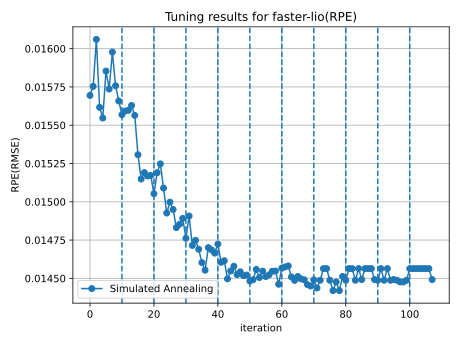
\includegraphics[width=0.75\linewidth]{images/faster-lio-sa.pdf}
    \caption{RPE per iteration of Simulated Annealing}
\end{figure}

\section{fast-livo2}

\section{Possible improvements}